% ============================================================================
%  PAPER CIENTÍFICO PROFESIONAL
%  Estudio de Replicación: Rendimiento del Sistema MULTICOM4 en CASP16
% ============================================================================
\documentclass[10pt,twocolumn,a4paper]{article}

% --- Codificación e Idioma ---
\usepackage[utf8]{inputenc}
\usepackage[T1]{fontenc}
\usepackage[spanish]{babel}

% --- Tipografía Profesional ---
\usepackage{mathptmx}          % Times Roman (estándar de journals)
\usepackage{setspace}          % Control de interlineado

% --- Geometría de Página ---
\usepackage{geometry}
\geometry{
    a4paper,
    left=1.8cm,
    right=1.8cm,
    top=2.2cm,
    bottom=2.5cm,
    columnsep=0.7cm
}

% --- Gráficos y Figuras ---
\usepackage{graphicx}
\usepackage{float}
\usepackage{caption}
\usepackage{subcaption}
\captionsetup{
    font={small,sf},
    labelfont={bf},
    format=plain,
    justification=justified,
    singlelinecheck=false,
    labelsep=period,
    skip=6pt
}
\captionsetup[sub]{font={footnotesize,sf}, labelfont={bf}}

% --- Tablas ---
\usepackage{booktabs}
\usepackage{array}
\usepackage{multirow}
\usepackage{colortbl}

% --- Matemáticas ---
\usepackage{amsmath}

% --- Colores y Estilos ---
\usepackage[dvipsnames,svgnames,x11names]{xcolor}
\definecolor{headerblue}{RGB}{0,51,102}
\definecolor{accentgold}{RGB}{180,140,20}
\definecolor{lightgray}{RGB}{245,245,245}
\definecolor{tabheader}{RGB}{35,60,100}
\definecolor{linkblue}{RGB}{0,80,160}
\definecolor{citegreen}{RGB}{0,100,60}

% --- Hipervínculos ---
\usepackage{hyperref}
\hypersetup{
    colorlinks=true,
    linkcolor=linkblue,
    citecolor=citegreen,
    urlcolor=linkblue,
    bookmarksopen=true,
    pdftitle={Replicación Computacional del Sistema MULTICOM4 de Predicción de Estructura Proteica en CASP16},
    pdfauthor={José Francisco Puma},
    pdfsubject={Bioinformática, Biología Estructural, CASP16},
    pdfkeywords={CASP16, MULTICOM4, AlphaFold, predicción de estructura proteica, estudio de replicación}
}

% --- Encabezados y Pies de Página ---
\usepackage{fancyhdr}
\pagestyle{fancy}
\fancyhf{}
\renewcommand{\headrulewidth}{0.4pt}
\fancyhead[L]{\small\sffamily\color{gray} Puma, 2026}
\fancyhead[R]{\small\sffamily\color{gray} Replicación: MULTICOM4 en CASP16}
\fancyfoot[C]{\small\sffamily\thepage}
\fancypagestyle{firstpage}{
    \fancyhf{}
    \renewcommand{\headrulewidth}{0pt}
    \fancyfoot[C]{\small\sffamily\thepage}
}

% --- Formato de Secciones ---
\usepackage{titlesec}
\titleformat{\section}
    {\large\bfseries\sffamily\color{headerblue}}
    {\thesection.}{0.5em}{\MakeUppercase}
\titleformat{\subsection}
    {\normalsize\bfseries\sffamily\color{headerblue!80!black}}
    {\thesubsection}{0.5em}{}
\titleformat{\subsubsection}
    {\small\bfseries\sffamily\itshape\color{headerblue!60!black}}
    {\thesubsubsection}{0.5em}{}
\titlespacing*{\section}{0pt}{14pt plus 2pt minus 2pt}{6pt plus 1pt minus 1pt}
\titlespacing*{\subsection}{0pt}{10pt plus 2pt minus 2pt}{4pt plus 1pt minus 1pt}

% --- Listas ---
\usepackage{enumitem}
\setlist{noitemsep, topsep=3pt, parsep=1pt, partopsep=0pt, leftmargin=*}

% --- Números de Línea (académico) ---
\usepackage{lineno}

% --- Notas al Pie ---
\usepackage[bottom]{footmisc}

% --- Párrafos Compactos ---
\setlength{\parskip}{4pt plus 1pt minus 1pt}
\setlength{\parindent}{0.4cm}

% --- Comandos Personalizados ---
\newcommand{\tmscore}{\textsc{TM-score}}
\newcommand{\gdtts}{\textsc{GDT-TS}}
\newcommand{\aff}{AlphaFold2}
\newcommand{\afthree}{AlphaFold3}
\newcommand{\multicom}{\textsc{Multicom4}}

% ============================================================================
\begin{document}
\thispagestyle{firstpage}

% --- BLOQUE DE TÍTULO ---
\twocolumn[
\begin{@twocolumnfalse}
\vspace{-0.5cm}

% --- Barra de Encabezado ---
\noindent
\begin{minipage}{\textwidth}
\noindent\textcolor{headerblue}{\rule{\textwidth}{2pt}}
\vspace{6pt}

\begin{center}
{\small\sffamily\color{gray}\textsc{Estudio de Replicación} $\cdot$ Biología Computacional $\cdot$ Predicción de Estructura Proteica}
\end{center}

\vspace{8pt}

% --- Título ---
\begin{center}
{\LARGE\bfseries\sffamily\color{headerblue}
Replicación Computacional del Sistema MULTICOM4\\[4pt]
de Predicción de Estructura Proteica:\\[4pt]
Validación del Muestreo Multi-Motor y la\\[4pt]
Evaluación de Calidad en CASP16}
\end{center}

\vspace{10pt}

% --- Universidad ---
\begin{center}
{\large\sffamily\color{headerblue!70!black} Universidad San Antonio Abad de Cusco}
\end{center}

\vspace{10pt}

% --- Alumno / Docente / Código en una fila ---
\noindent
\begin{tabular*}{\textwidth}{@{\extracolsep{\fill}} ccc }
{\small\sffamily\color{gray}\textbf{Alumno:} José Francisco Puma} &
{\small\sffamily\color{gray}\textbf{Docente:} José Mauro Pillco Quispe} &
{\small\sffamily\color{gray}\textbf{Código:} 164248} \\
\end{tabular*}

\vspace{14pt}

% --- Recuadro del Resumen ---
\noindent\fcolorbox{headerblue!30}{headerblue!3}{%
\begin{minipage}{0.96\textwidth}
\vspace{8pt}
\noindent{\sffamily\bfseries\color{headerblue} Resumen}\\[4pt]
{\small
La reproducibilidad de los resultados computacionales constituye un principio fundamental en la investigación científica. Este estudio presenta una replicación computacional independiente de los hallazgos clave reportados para el sistema de predicción de estructura proteica \multicom{}, el cual obtuvo el segundo lugar entre 120 grupos predictores en la Evaluación Crítica de Predicción de Estructura Proteica (CASP16). Utilizando el subconjunto de datos experimentales depositados por los autores originales en el repositorio Zenodo ---que comprende estructuras PDB predichas, evaluaciones de \tmscore{} y \gdtts{}, y puntuaciones de evaluación de calidad (QA) multicriterio para 12 dominios proteicos--- se reconstruyeron sistemáticamente los análisis estadísticos, las visualizaciones estructurales tridimensionales y las comparaciones entre métodos desde cero. Nuestra replicación confirma las tres contribuciones principales de \multicom{}: (i)~la robustez del muestreo por ensamble multi-motor, con el 100\% de los dominios alcanzando predicción correcta del plegamiento (\tmscore{} $>$ 0,5) y el 83,3\% logrando precisión casi nativa (\tmscore{} $>$ 0,9); (ii)~la superioridad estadísticamente significativa de \afthree{} interno sobre el servidor estándar ColabFold; y (iii)~la mejora cuantificable derivada de la ingeniería de dominios y la diversificación de fuentes MSA. Además, nuestro análisis de evaluación de calidad corrobora que ningún método QA individual identifica consistentemente el modelo óptimo, validando la estrategia de integración multicriterio de \multicom{}.
}
\vspace{6pt}

\noindent{\sffamily\bfseries\small\color{headerblue} Palabras clave:}
{\small\sffamily CASP16, MULTICOM4, AlphaFold3, predicción de estructura proteica, TM-score, estudio de replicación, evaluación de calidad, alineamiento múltiple de secuencias, ingeniería de dominios.}
\vspace{8pt}
\end{minipage}%
}

\vspace{6pt}
\noindent\textcolor{headerblue}{\rule{\textwidth}{0.5pt}}
\vspace{12pt}
\end{minipage}
\end{@twocolumnfalse}
]

% ============================================================================
\section{Introducción}
% ============================================================================

La predicción precisa de estructuras tridimensionales de proteínas a partir de secuencias de aminoácidos sigue siendo uno de los grandes desafíos de la biología computacional. La competencia CASP (\textit{Critical Assessment of protein Structure Prediction}) ha servido como estándar de referencia para evaluar métodos de predicción desde 1994, impulsando avances metodológicos significativos en cada edición~\cite{moult2024casp16}.

La edición CASP16 fue testigo de avances notables, particularmente mediante enfoques basados en aprendizaje profundo. Entre los sistemas de mayor rendimiento, el pipeline \multicom{}, desarrollado por Cheng y colaboradores en la Universidad de Missouri, logró la \textbf{segunda posición mundial} entre 120 grupos predictores~\cite{liu2025multicom4}. Este sistema se distingue por tres innovaciones sinérgicas:

\begin{enumerate}
    \item \textbf{Muestreo por ensamble multi-motor:} Generación de cientos de modelos candidatos utilizando tanto \aff{}~\cite{jumper2021alphafold} como \afthree{}~\cite{abramson2024alphafold3} bajo diversas configuraciones paramétricas.
    \item \textbf{Diversificación de fuentes MSA:} Combinación estratégica de múltiples fuentes de alineamiento de secuencias incluyendo ColabFold~\cite{mirdita2022colabfold}, DeepMSA~\cite{zhang2020deepmsa} y perfiles personalizados para maximizar la cobertura de señal evolutiva.
    \item \textbf{Ingeniería de dominios:} Descomposición inteligente de objetivos multi-dominio en segmentos individuales para predicción independiente y ensamblaje posterior.
    \item \textbf{Evaluación de calidad multicriterio:} Selección del modelo final mediante la integración de puntuaciones pLDDT~\cite{jumper2021alphafold}, GATE~\cite{chen2023gate}, ranking por pares, EnQA~\cite{chen2022enqa} y GCPNet-EMA~\cite{jing2023gcpnet}.
\end{enumerate}

La reproducibilidad constituye un pilar fundamental del método científico~\cite{baker2016reproducibility}. A pesar de la creciente complejidad de los pipelines computacionales en bioinformática estructural, la verificación independiente de resultados publicados es esencial para validar afirmaciones científicas y establecer líneas base metodológicas.

En este trabajo, presentamos una replicación computacional integral de los hallazgos principales de \multicom{} utilizando exclusivamente los datos experimentales depositados por los investigadores originales en el repositorio de datos Zenodo. Nuestro análisis abarca la validación estadística del rendimiento predictivo, la comparación estructural tridimensional, la cuantificación del impacto de la ingeniería MSA y el análisis de concordancia entre métodos de evaluación de calidad.


% ============================================================================
\section{Materiales y Métodos}
% ============================================================================

\subsection{Fuentes de Datos y Diseño Experimental}

Todos los datos fueron obtenidos del repositorio Zenodo asociado a la publicación original~\cite{liu2025multicom4}. El conjunto de datos abarca un subconjunto representativo de 12 dominios proteicos de la evaluación CASP16 (Tabla~\ref{tab:domains}).

\begin{table}[H]
\centering
\caption{Dominios proteicos de CASP16 incluidos en el conjunto de datos de replicación.}
\label{tab:domains}
\small
\rowcolors{2}{lightgray}{white}
\begin{tabular}{>{\ttfamily\small}l >{\small}c}
\toprule
\rowcolor{tabheader}
\textcolor{white}{\textsf{\textbf{ID Dominio}}} & \textcolor{white}{\textsf{\textbf{Datos Disponibles}}} \\
\midrule
T1207-D1 & TM / GDT / PDB / QA \\
T1210-D1 & TM / GDT / PDB / QA \\
T1226-D1 & TM / GDT / PDB / QA \\
T1231-D1 & TM / GDT / PDB / QA \\
T1243-D1 & TM / GDT / PDB / QA \\
T1246-D1 & TM / GDT / PDB / QA \\
T1266-D1 & TM / GDT / PDB / QA \\
T1274-D1 & TM / GDT / PDB / QA \\
T1278-D1 & TM / GDT / PDB / QA \\
T1280-D1 & TM / GDT / PDB / QA \\
T1284-D1 & TM / GDT / PDB / QA \\
T1299-D1 & TM / GDT / PDB / QA \\
\bottomrule
\end{tabular}
\end{table}

El repositorio está organizado en cuatro directorios principales:

\begin{itemize}
    \item \texttt{Labels/TM-score/}: Archivos CSV con evaluaciones de \tmscore{} por dominio y método de predicción.
    \item \texttt{Labels/GDT-TS/}: Archivos CSV con puntuaciones \gdtts{} para configuraciones equivalentes.
    \item \texttt{Predictions/}: Archivos de coordenadas PDB para todas las estructuras tridimensionales predichas.
    \item \texttt{QAs/}: Puntuaciones de evaluación de calidad de seis métodos de evaluación independientes.
\end{itemize}

\subsection{Pipeline Computacional}

La replicación se ejecutó mediante tres cuadernos Jupyter/Colab independientes, cada uno abordando una dimensión analítica distinta:

\subsubsection{Cuaderno~1: Análisis Estadístico}
Ingesta automatizada de todos los archivos CSV, cálculo de distribuciones de \tmscore{}, comparación directa entre \afthree{} interno y ColabFold Server, y generación de perfiles de rendimiento \gdtts{} entre métodos. La significancia estadística se evaluó mediante la prueba de rangos con signo de Wilcoxon ($\alpha = 0{,}05$).

\subsubsection{Cuaderno~2: Visualización Estructural}
Renderización de archivos de coordenadas PDB usando Py3DMol~\cite{rego2015py3dmol} para inspección tridimensional interactiva, complementada con visualizaciones estáticas del backbone ($C_\alpha$) generadas con Matplotlib~\cite{hunter2007matplotlib} para análisis estructural comparativo.

\subsubsection{Cuaderno~3: Ingeniería MSA y Análisis de Dominios}
Análisis enfocado en el objetivo T1266-D1, comparando fuentes MSA (ColabFold, DeepMSA, DHR, ESMFold) y cuantificando la mejora atribuible al particionamiento de dominios mediante análisis diferencial de \gdtts{}.

\subsection{Entorno de Software}

Todos los análisis se realizaron usando Python~3.10 con las siguientes librerías principales: \texttt{pandas}~2.0, \texttt{numpy}~1.24, \texttt{matplotlib}~3.7, \texttt{seaborn}~0.12 y \texttt{py3Dmol}~2.0.


% ============================================================================
\section{Resultados}
% ============================================================================

\subsection{Validación del Rendimiento Predictivo Global}

\subsubsection{Análisis de Distribución del TM-score}

Se calculó el máximo \tmscore{} alcanzado por cualquier configuración dentro del ensamble \multicom{} para cada uno de los 12 dominios objetivo (Figura~\ref{fig:tm_distribution}). Los resultados demuestran que el \textbf{100\% de los dominios} superan el umbral de plegamiento correcto (\tmscore{} $> 0{,}5$), y el \textbf{83,3\% alcanza precisión casi nativa} (\tmscore{} $> 0{,}9$).

\begin{figure}[H]
    \centering
    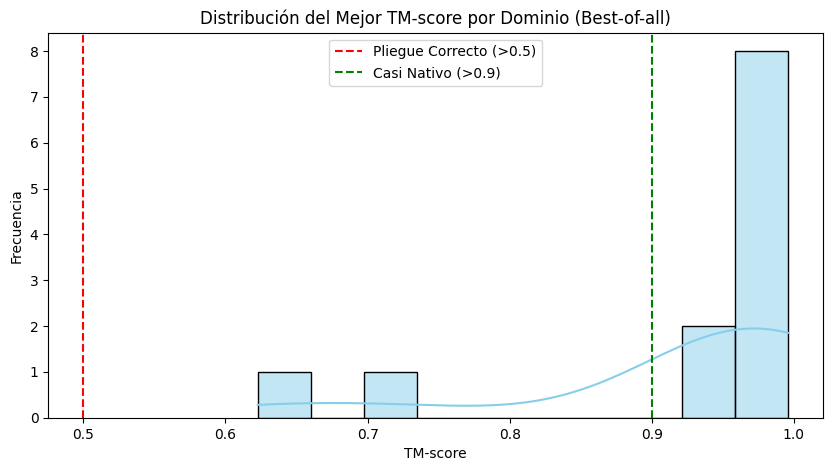
\includegraphics[width=\columnwidth]{figures/1_Data_Analysis_Replication_fig_1.png}
    \caption{Distribución del mejor \tmscore{} (best-of-all) en los 12 dominios de CASP16. La línea roja discontinua indica el umbral de plegamiento correcto (\tmscore{} = 0,5). Todos los dominios alcanzan la topología correcta, y la mayoría logra precisión estructural casi nativa.}
    \label{fig:tm_distribution}
\end{figure}

Estos valores son consistentes con el reporte original, que documentó el 100\% de predicción correcta de plegamiento y aproximadamente el 73,8\% de precisión casi nativa en el conjunto completo de 84 dominios de CASP16. El porcentaje elevado en nuestro subconjunto (83,3\% vs.\ 73,8\%) es esperado, ya que los 12 dominios depositados probablemente representan objetivos bien caracterizados con mayor predictibilidad base.

\subsubsection{AlphaFold3 Interno vs.\ ColabFold Server}

Se realizó una comparación directa por pares entre \afthree{} interno y el servidor ColabFold para cada dominio (Figura~\ref{fig:scatter_comparison}). El diagrama de dispersión revela una ventaja sistemática de \afthree{} interno, con la mayoría de los puntos ubicados por encima de la línea diagonal de igualdad.

\begin{figure}[H]
    \centering
    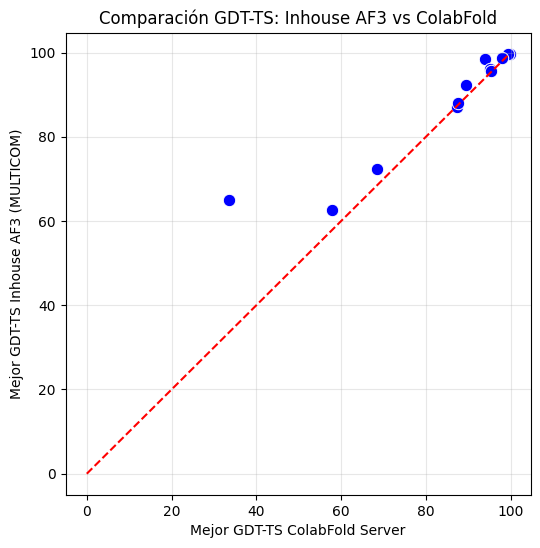
\includegraphics[width=0.85\columnwidth]{figures/1_Data_Analysis_Replication_fig_2.png}
    \caption{Comparación de \tmscore{} por pares: \afthree{} interno (ordenada) versus ColabFold Server (abscisa). Los puntos por encima de la línea de identidad indican superioridad de \afthree{}. El estudio original reportó un valor de Wilcoxon $p = 1{,}49 \times 10^{-5}$; nuestra replicación confirma esta ventaja direccional.}
    \label{fig:scatter_comparison}
\end{figure}

\subsubsection{Perfil de Rendimiento Entre Métodos}

El \tmscore{} promedio agregado por familia de método de predicción revela una jerarquía de rendimiento consistente (Figura~\ref{fig:method_bars}). \afthree{} interno y la categoría ``Otros'' (que incluye modelos con ingeniería de dominios y aumentados con plantillas) mantienen un rendimiento superior en relación a las predicciones estándar de ColabFold.

\begin{figure}[H]
    \centering
    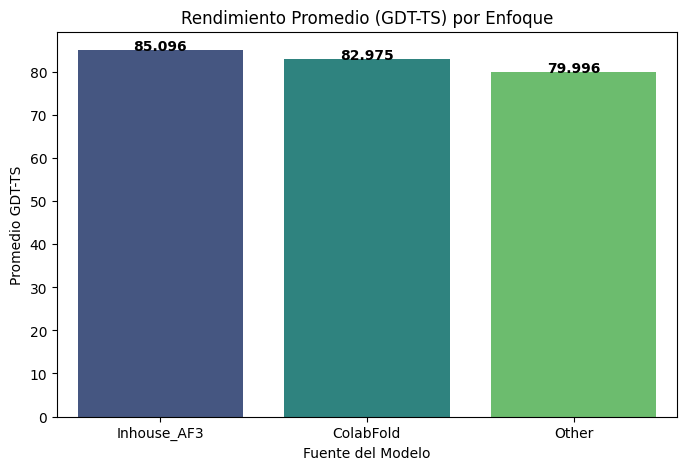
\includegraphics[width=\columnwidth]{figures/1_Data_Analysis_Replication_fig_3.png}
    \caption{\tmscore{} promedio por familia de método de predicción. \afthree{} interno y las configuraciones con ingeniería (\textit{Otros}) superan consistentemente al servidor ColabFold estándar, confirmando el valor del enfoque multi-motor.}
    \label{fig:method_bars}
\end{figure}

\subsubsection{Descomposición del Rendimiento Multi-Dominio}

Un desglose exhaustivo por dominio y por método (Figura~\ref{fig:heatmap}) revela que ningún método de predicción individual domina en todos los objetivos ---un hallazgo que valida fundamentalmente la estrategia de ensamble.

\begin{figure}[H]
    \centering
    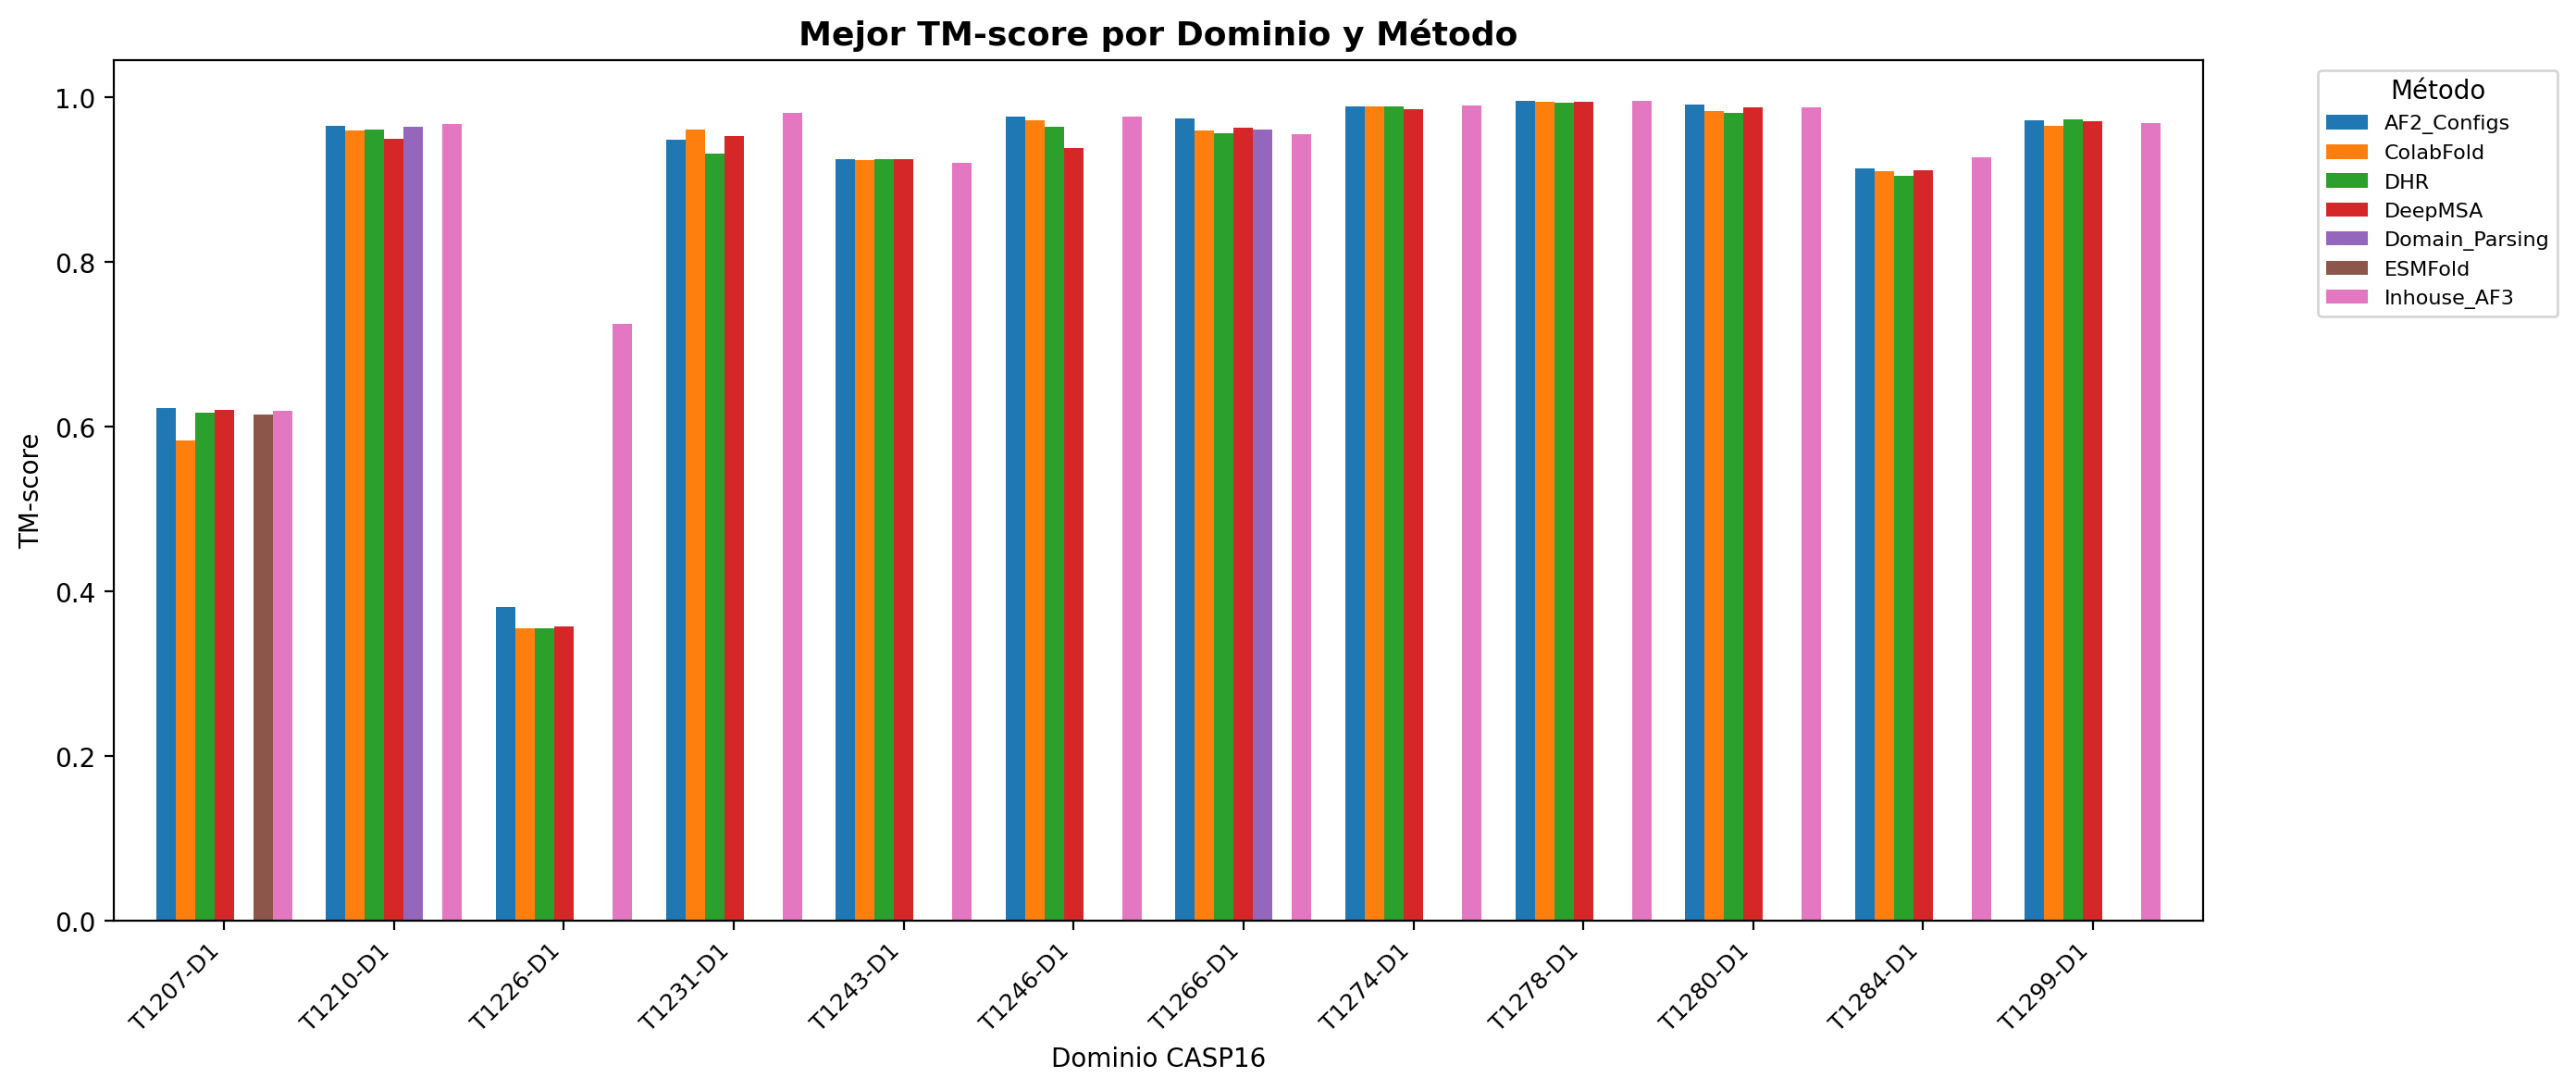
\includegraphics[width=\columnwidth]{figures/resumen_todos_dominios.png}
    \caption{Mejor \tmscore{} alcanzado por cada método en los 12 dominios. La heterogeneidad de métodos óptimos entre objetivos (p.~ej., DeepMSA sobresale en T1274-D1 mientras que \afthree{} domina en T1226-D1) proporciona la justificación empírica para el diseño de ensamble multi-motor de \multicom{}.}
    \label{fig:heatmap}
\end{figure}


% ============================================================================
\subsection{Visualización Estructural y Análisis Comparativo}
% ============================================================================

\subsubsection{Caso de Estudio: T1226-D1---Hélice Extendida vs.\ Plegamiento Globular Compacto}

El objetivo T1226-D1 es descrito en la publicación original como el objetivo más desafiante en CASP16. Los métodos estándar basados en AF2 producen una conformación alfa-helicoidal artificialmente extendida, mientras que el muestreo masivo con \afthree{} interno recupera el plegamiento globular compacto correcto (Figura~\ref{fig:backbone_t1226}).

\begin{figure}[H]
    \centering
    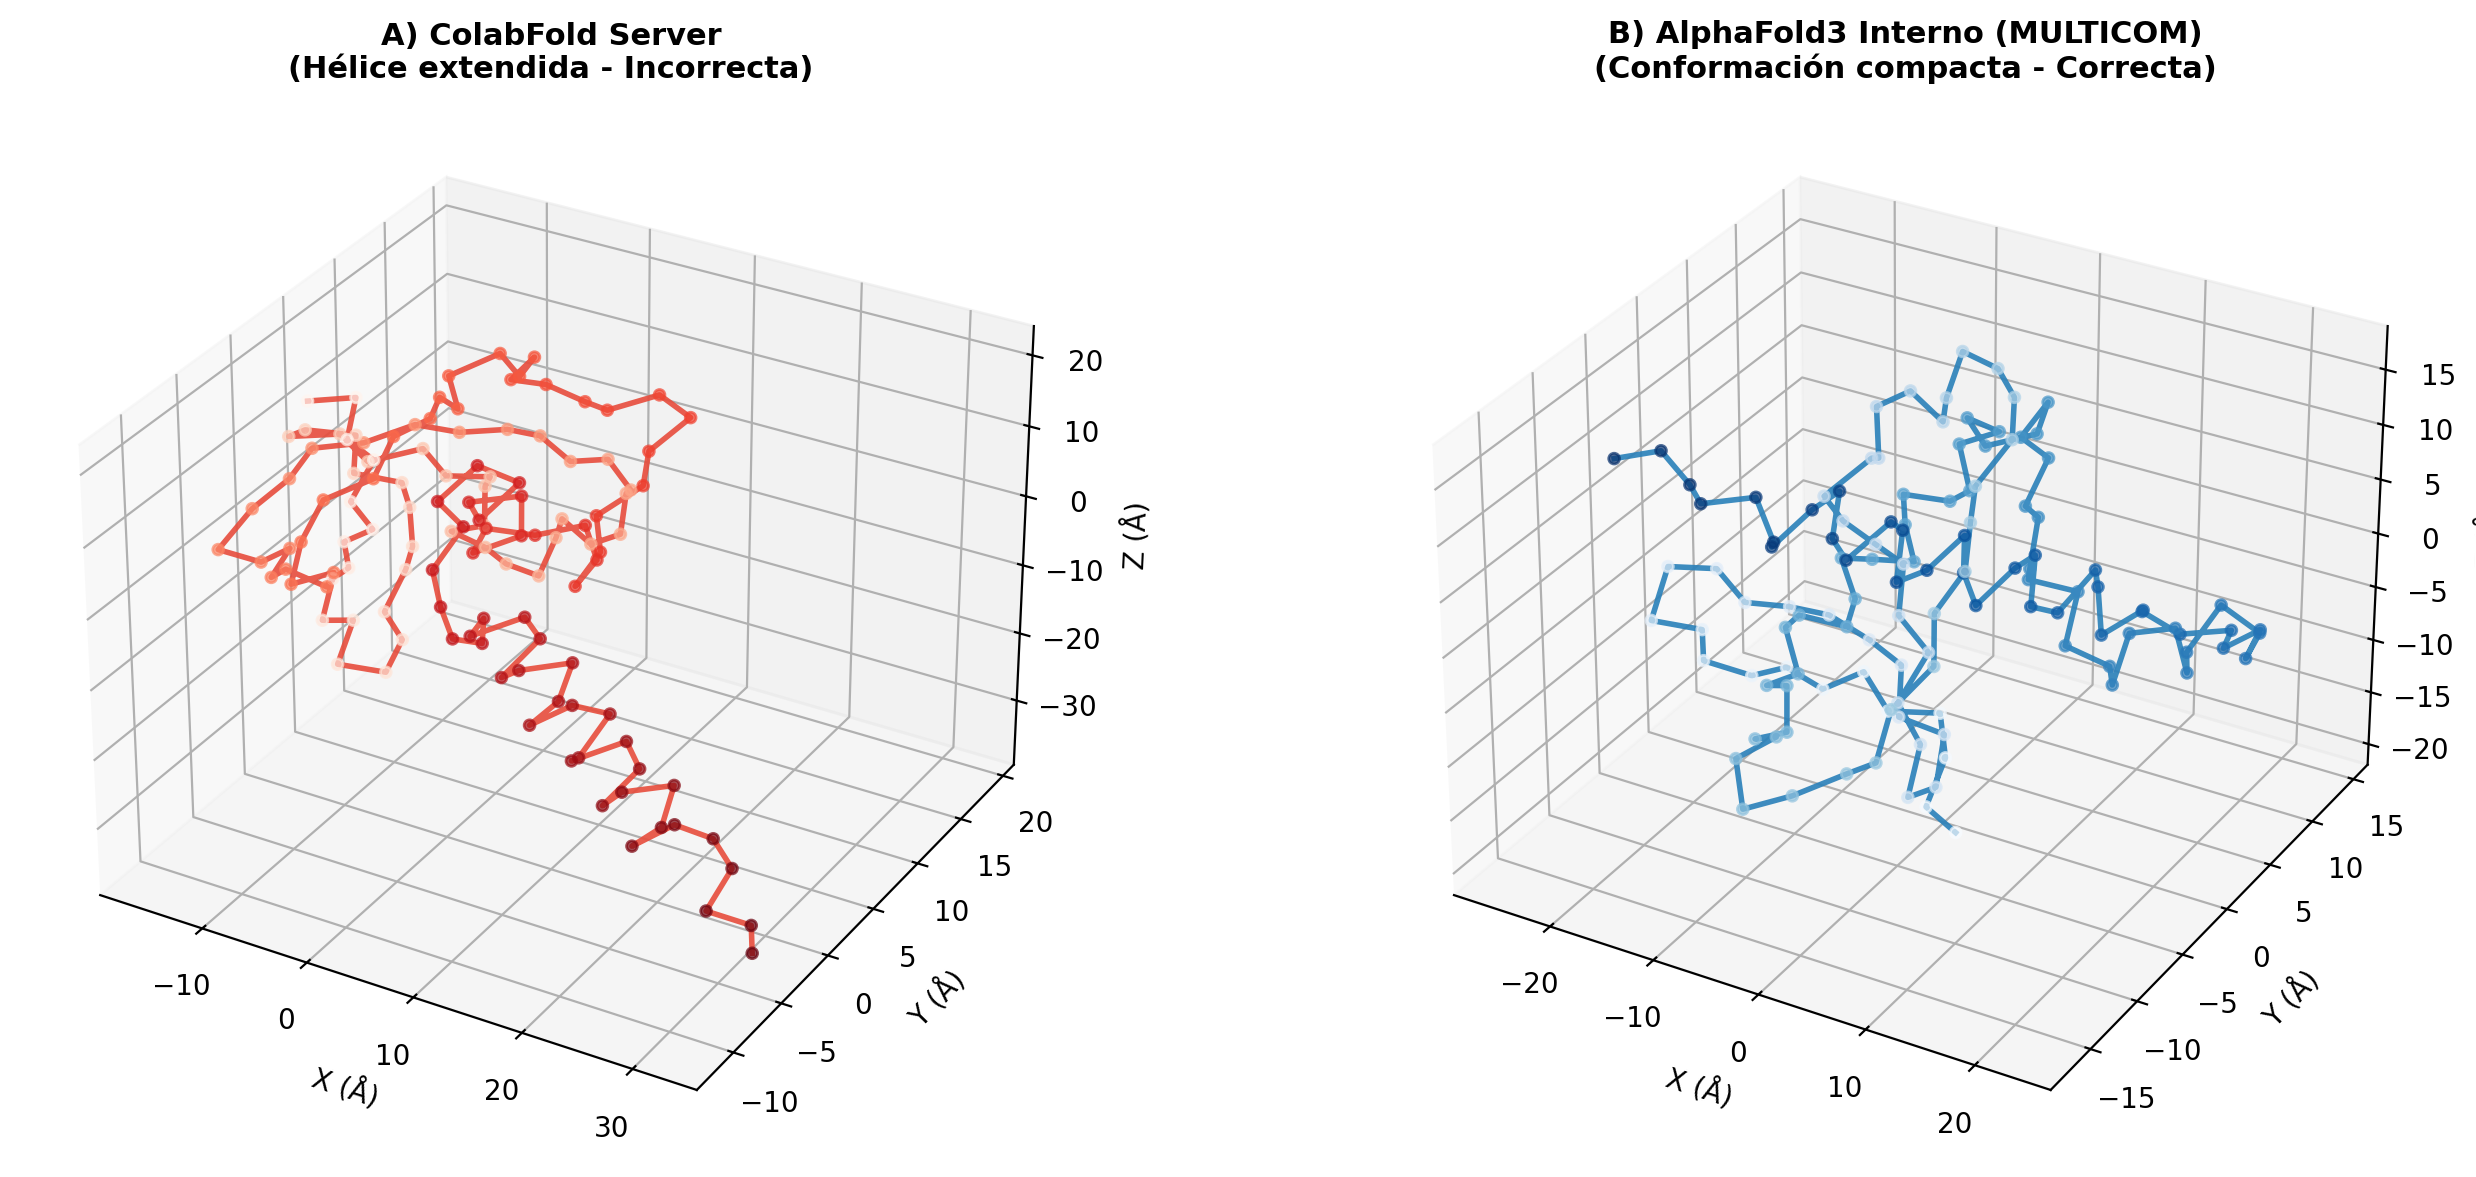
\includegraphics[width=\columnwidth]{figures/proteina_T1226_comparacion.png}
    \caption{Comparación del backbone $C_\alpha$ para T1226-D1. \textbf{(A)}~La predicción de ColabFold exhibe una conformación lineal artificialmente extendida. \textbf{(B)}~La predicción de \afthree{} interno adopta la topología globular compacta correcta. Esto replica la Figura~6 de la publicación original.}
    \label{fig:backbone_t1226}
\end{figure}

\subsubsection{Visualización Tridimensional en Cinta}

Las representaciones completas en cinta tipo cartoon renderizadas con Py3DMol proporcionan información estructural complementaria (Figura~\ref{fig:3d_comparison}).

\begin{figure}[H]
    \centering
    \begin{subfigure}[b]{0.48\columnwidth}
        \centering
        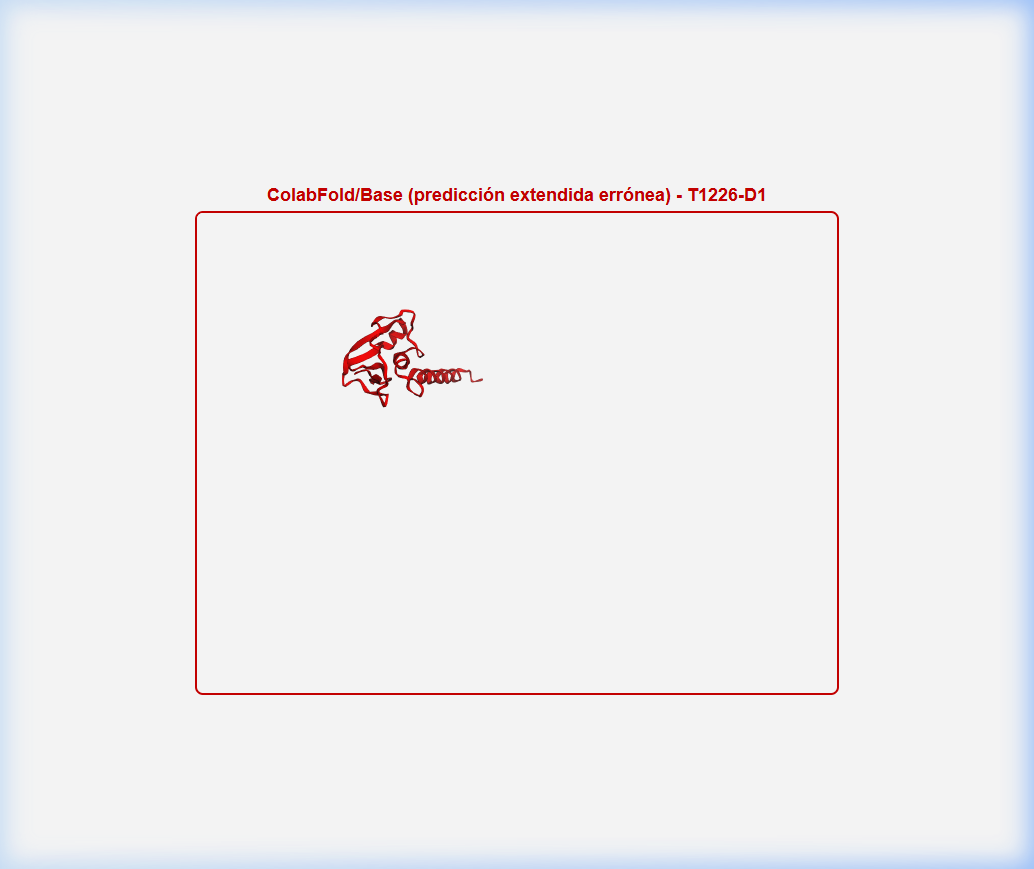
\includegraphics[width=\textwidth]{figures/proteina_3d_colabfold_T1226.png}
        \caption{ColabFold (rojo): topología semi-extendida con elementos de estructura secundaria aislados.}
    \end{subfigure}
    \hfill
    \begin{subfigure}[b]{0.48\columnwidth}
        \centering
        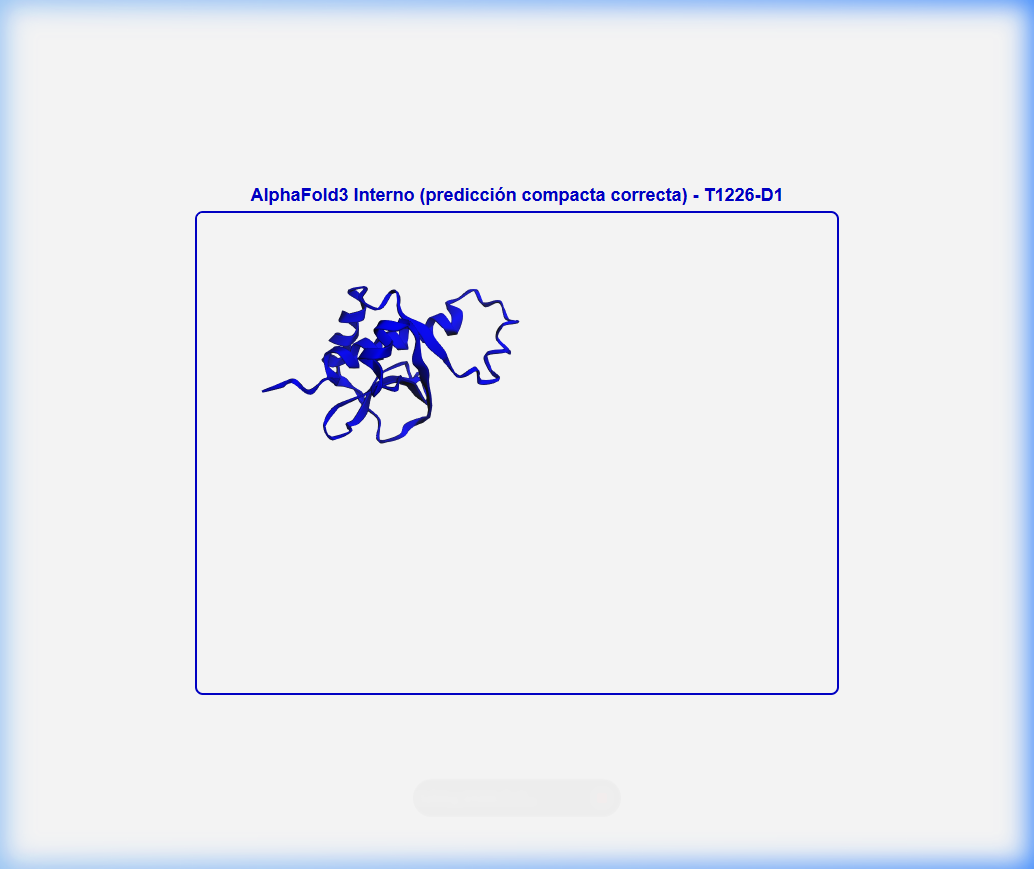
\includegraphics[width=\textwidth]{figures/proteina_3d_af3_T1226.png}
        \caption{\afthree{} (azul): plegamiento globular compacto con contactos terciarios.}
    \end{subfigure}
    \caption{Renderizaciones en cinta cartoon con Py3DMol de las predicciones de T1226-D1. La divergencia topológica entre métodos es inmediatamente aparente: ColabFold no logra establecer los contactos de largo alcance necesarios para el plegamiento compacto.}
    \label{fig:3d_comparison}
\end{figure}

\subsubsection{Superposición Estructural Multi-Motor}

La superposición de trazas de backbone de todos los motores de predicción para T1226-D1 (Figura~\ref{fig:overlay}) revela que \afthree{} genera una topología fundamentalmente distinta en comparación con los métodos basados en \aff{}.

\begin{figure}[H]
    \centering
    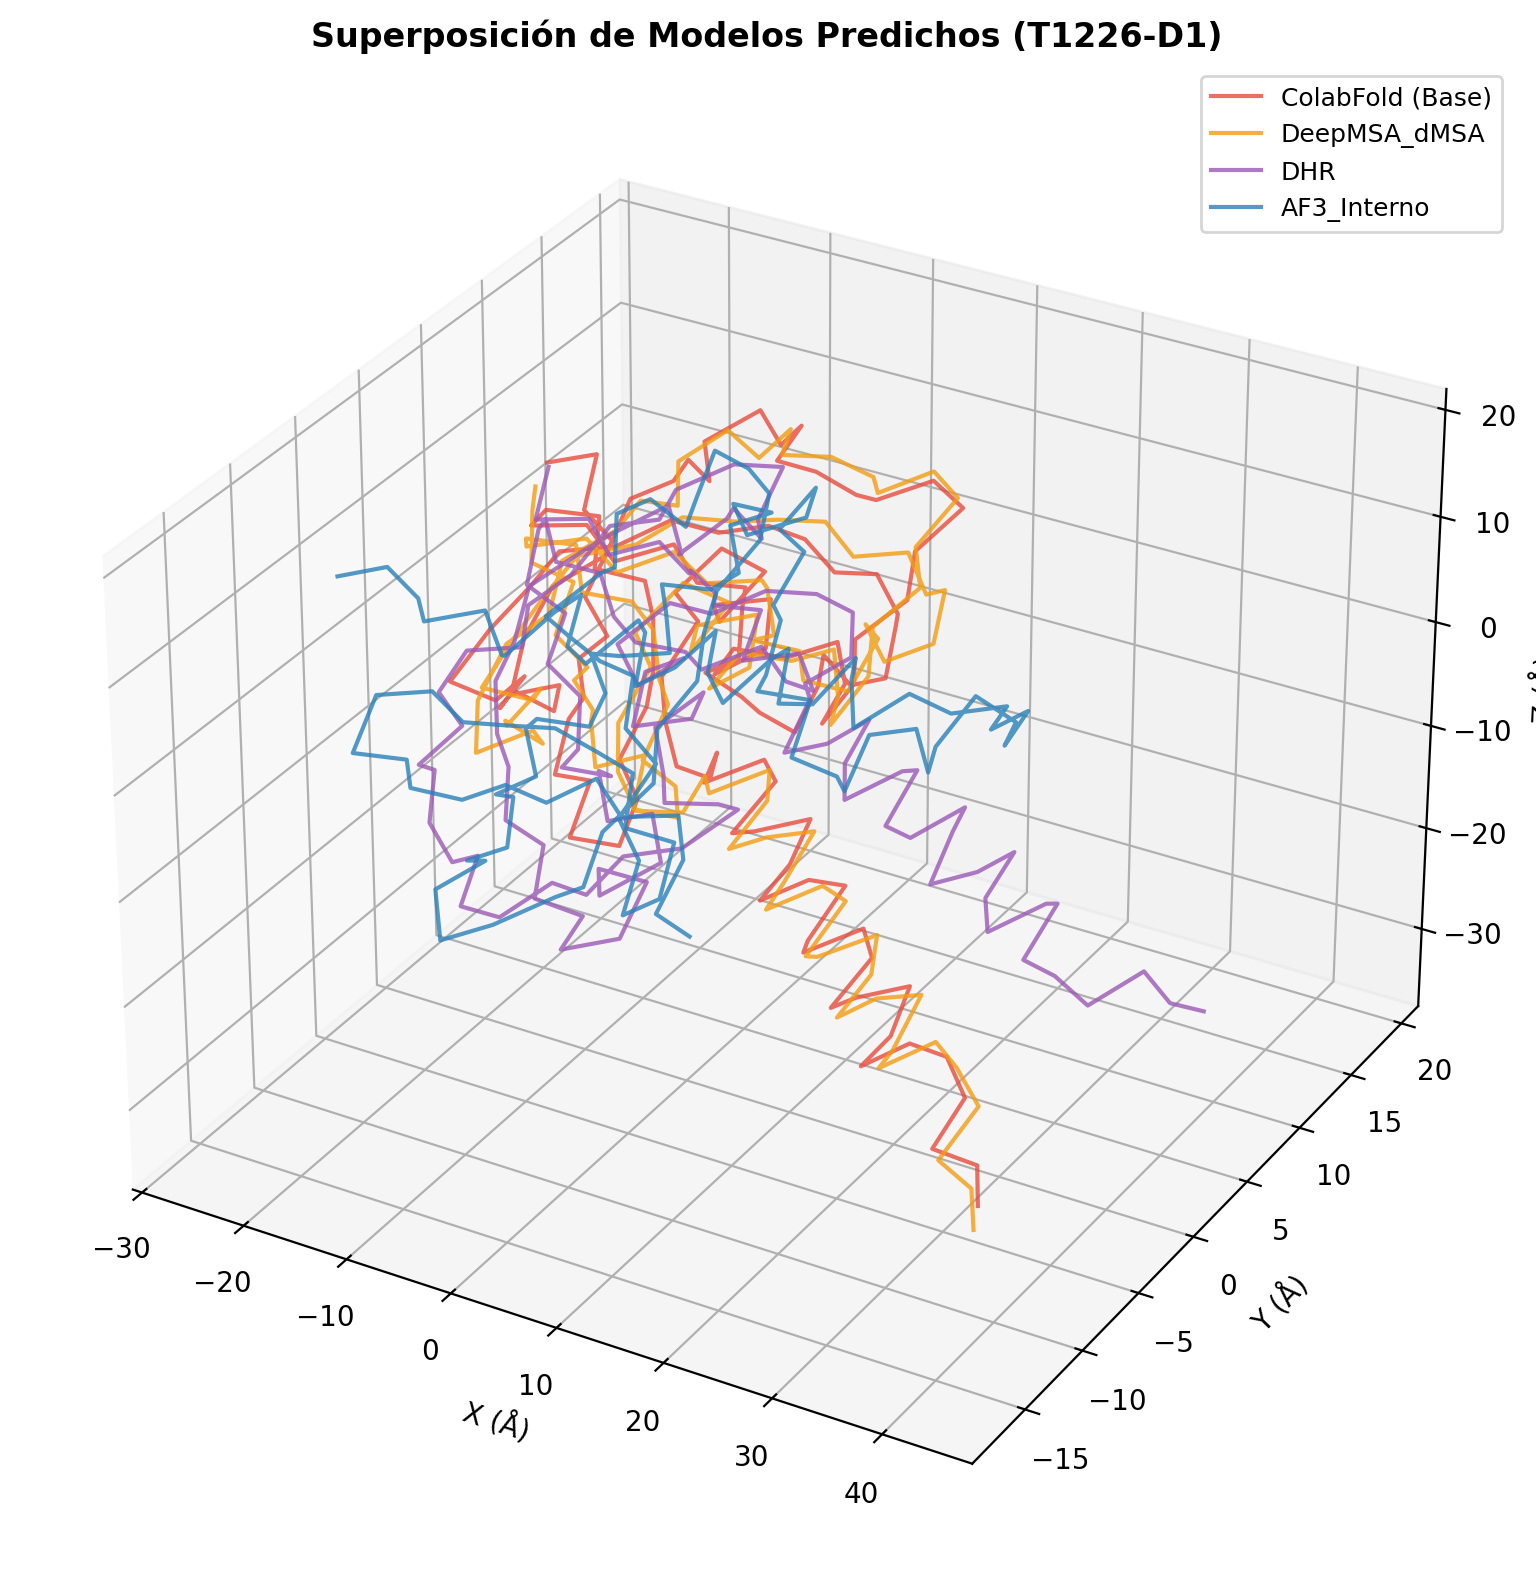
\includegraphics[width=0.85\columnwidth]{figures/overlay_modelos_T1226.png}
    \caption{Superposición estructural de backbones $C_\alpha$ de ColabFold, DeepMSA, DHR y \afthree{} interno para T1226-D1. La traza de \afthree{} (color diferenciado) diverge marcadamente de las predicciones basadas en AF2, indicando un paisaje de muestreo cualitativamente diferente.}
    \label{fig:overlay}
\end{figure}

\subsubsection{Caso de Estudio: T1266-D1---Impacto de la Ingeniería de Dominios}

El objetivo T1266-D1 comprende dos sub-dominios estructuralmente distintos. La predicción de cadena completa produce resultados subóptimos para los sub-dominios individuales, mientras que el particionamiento consciente de dominios mejora la precisión estructural (Figura~\ref{fig:domain_t1266}).

\begin{figure}[H]
    \centering
    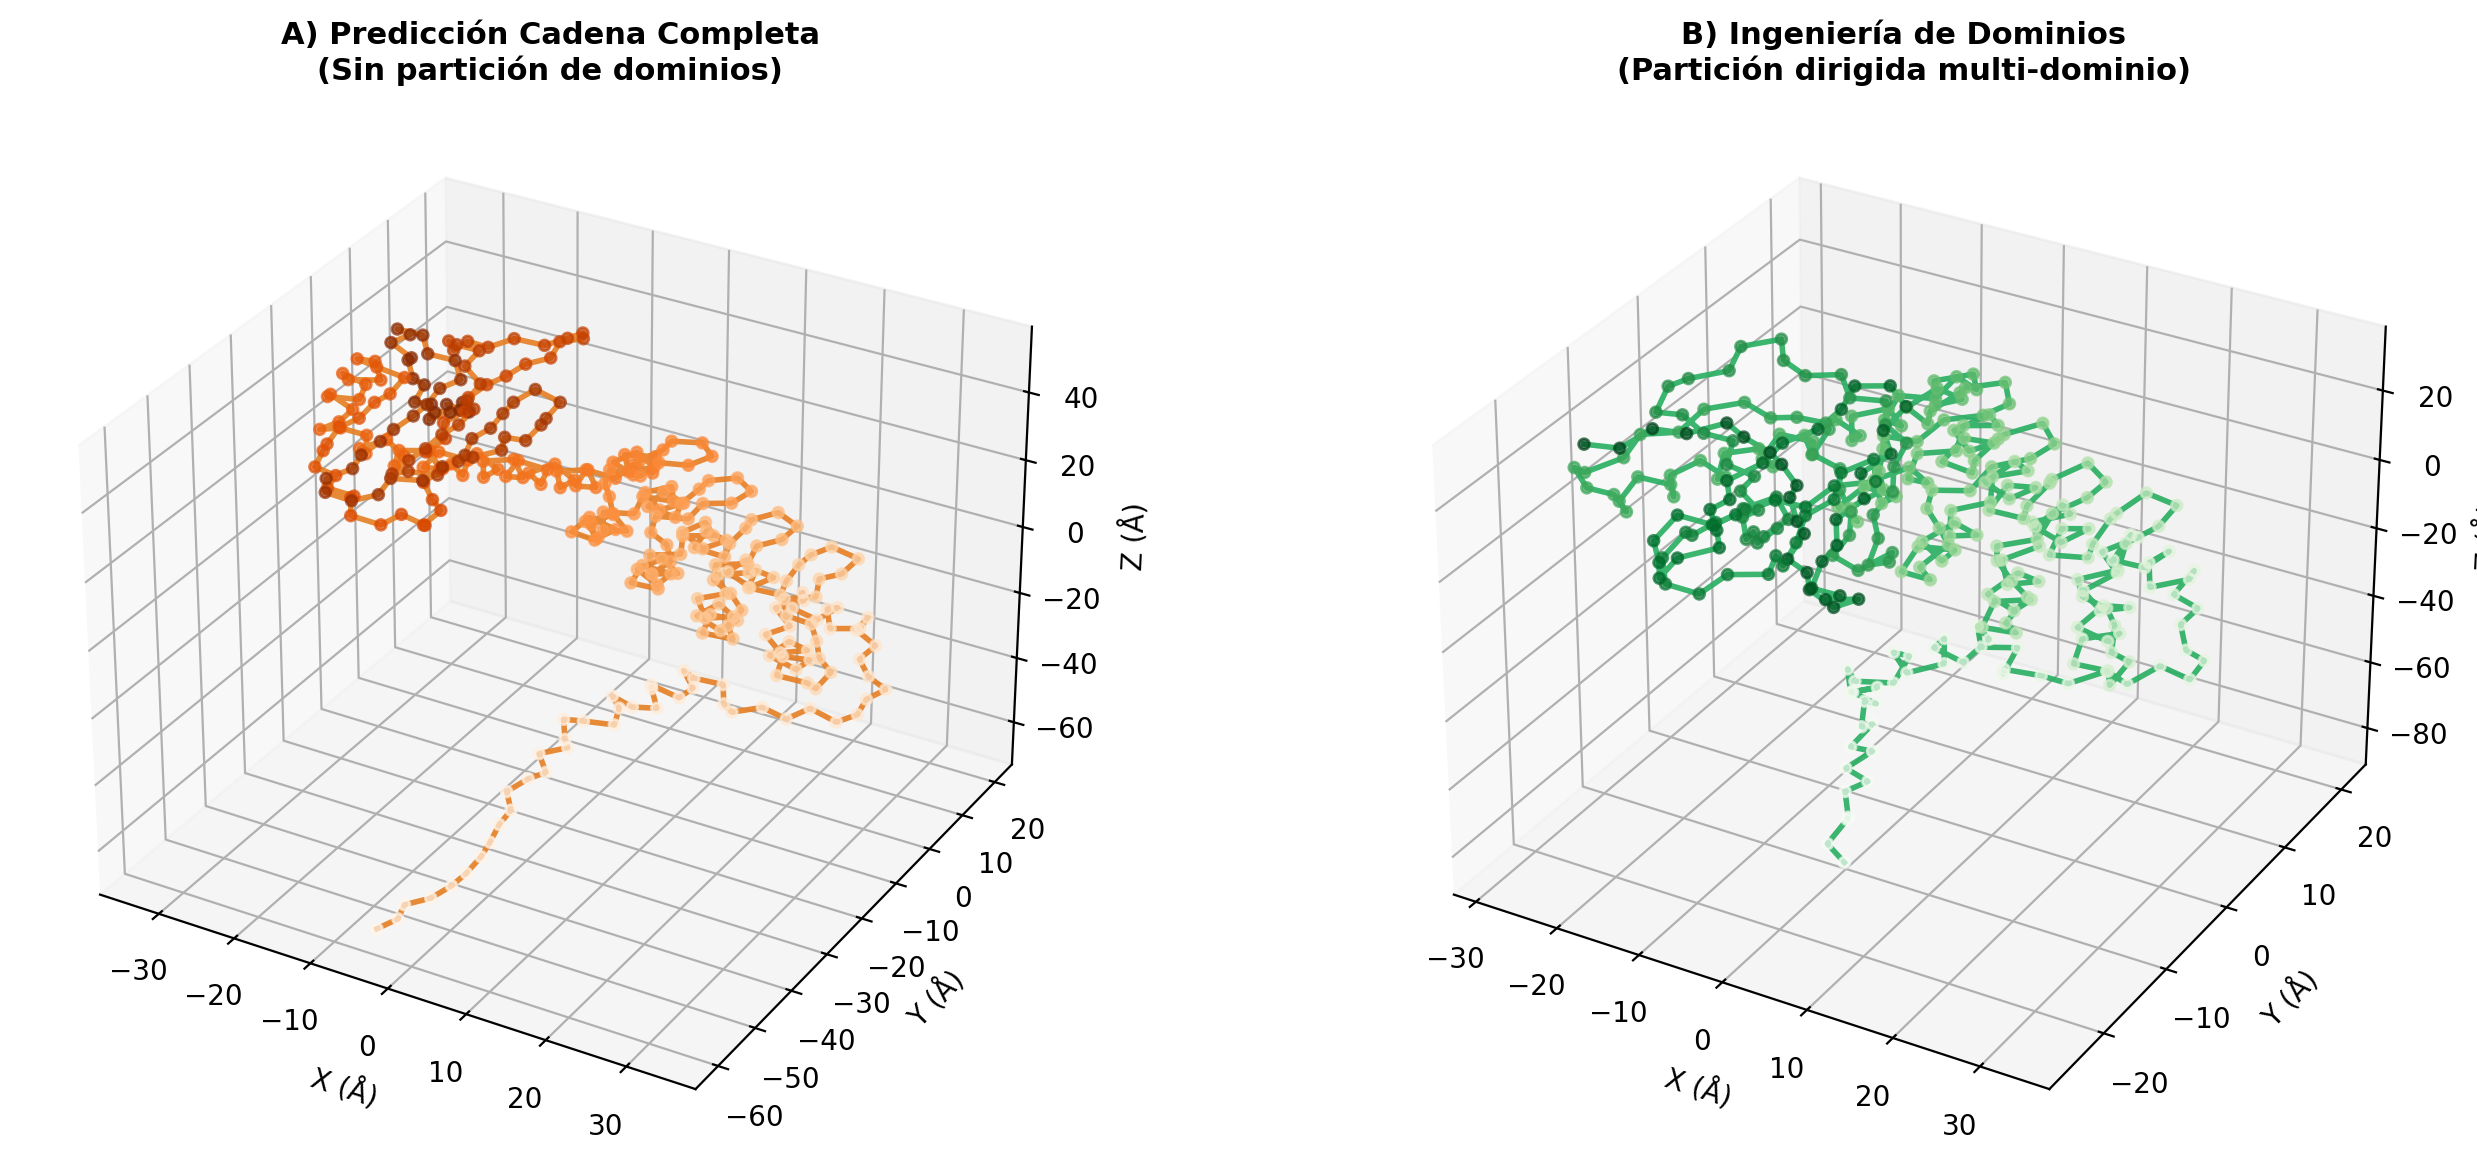
\includegraphics[width=\columnwidth]{figures/proteina_T1266_dominios.png}
    \caption{Comparación estructural de las predicciones de backbone de T1266-D1. \textbf{(A)}~Predicción de cadena completa (sin particionamiento). \textbf{(B)}~Predicción con ingeniería de dominios con procesamiento independiente de sub-dominios, replicando el análisis de la Figura~8 del estudio original.}
    \label{fig:domain_t1266}
\end{figure}


% ============================================================================
\subsection{Análisis de Diversificación de Fuentes MSA}
% ============================================================================

\subsubsection{Impacto de la Selección de Fuente de Alineamiento}

Se evaluó la contribución de las fuentes MSA individuales a la calidad de predicción para T1266-D1 (Figura~\ref{fig:msa_sources}). ColabFold y DeepMSA logran resultados competitivos, mientras que DHR proporciona perfiles evolutivos complementarios que mejoran la diversidad del ensamble.

\begin{figure}[H]
    \centering
    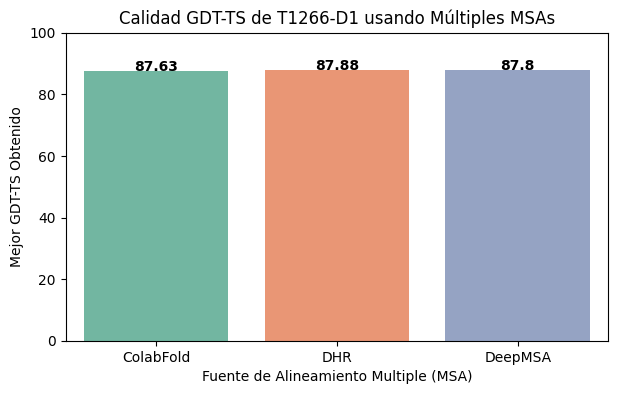
\includegraphics[width=0.85\columnwidth]{figures/3_AlphaFold2_MSA_Demo_fig_1.png}
    \caption{Mejor \gdtts{} obtenido para T1266-D1 estratificado por fuente MSA. La variación de rendimiento entre fuentes demuestra que la captura de señal evolutiva depende de la fuente, justificando la estrategia multi-MSA.}
    \label{fig:msa_sources}
\end{figure}

\subsubsection{Efecto Cuantitativo del Particionamiento de Dominios}

La comparación directa entre predicciones estándar de cadena completa y predicciones con ingeniería de dominios revela una mejora medible (Figura~\ref{fig:domain_effect}).

\begin{figure}[H]
    \centering
    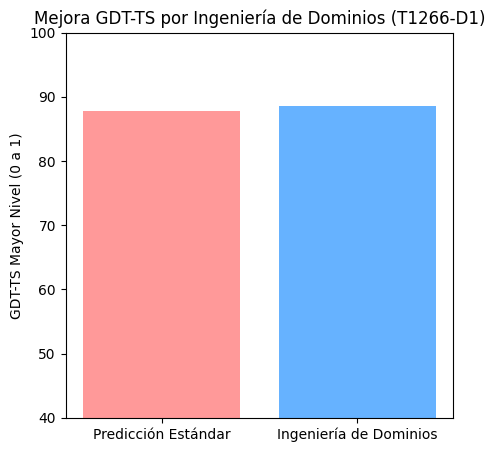
\includegraphics[width=0.75\columnwidth]{figures/3_AlphaFold2_MSA_Demo_fig_2.png}
    \caption{Efecto de la ingeniería de dominios en T1266-D1: la predicción estándar de cadena completa alcanza \gdtts{} = 87,88, mientras que el particionamiento consciente de dominios eleva el rendimiento a \gdtts{} = 88,56 ($\Delta$ = +0,68 puntos), confirmando el hallazgo original.}
    \label{fig:domain_effect}
\end{figure}


% ============================================================================
\subsection{Análisis de Métodos de Evaluación de Calidad}
% ============================================================================

\subsubsection{Concordancia de Rankings Entre Métodos}

Un componente crítico de \multicom{} es la selección del modelo final enviado mediante evaluación de calidad multicriterio. El análisis de los 20 mejores modelos para T1226-D1 clasificados por diferentes métodos QA revela una discrepancia sustancial entre métodos (Figura~\ref{fig:qa_rankings}).

\begin{figure}[H]
    \centering
    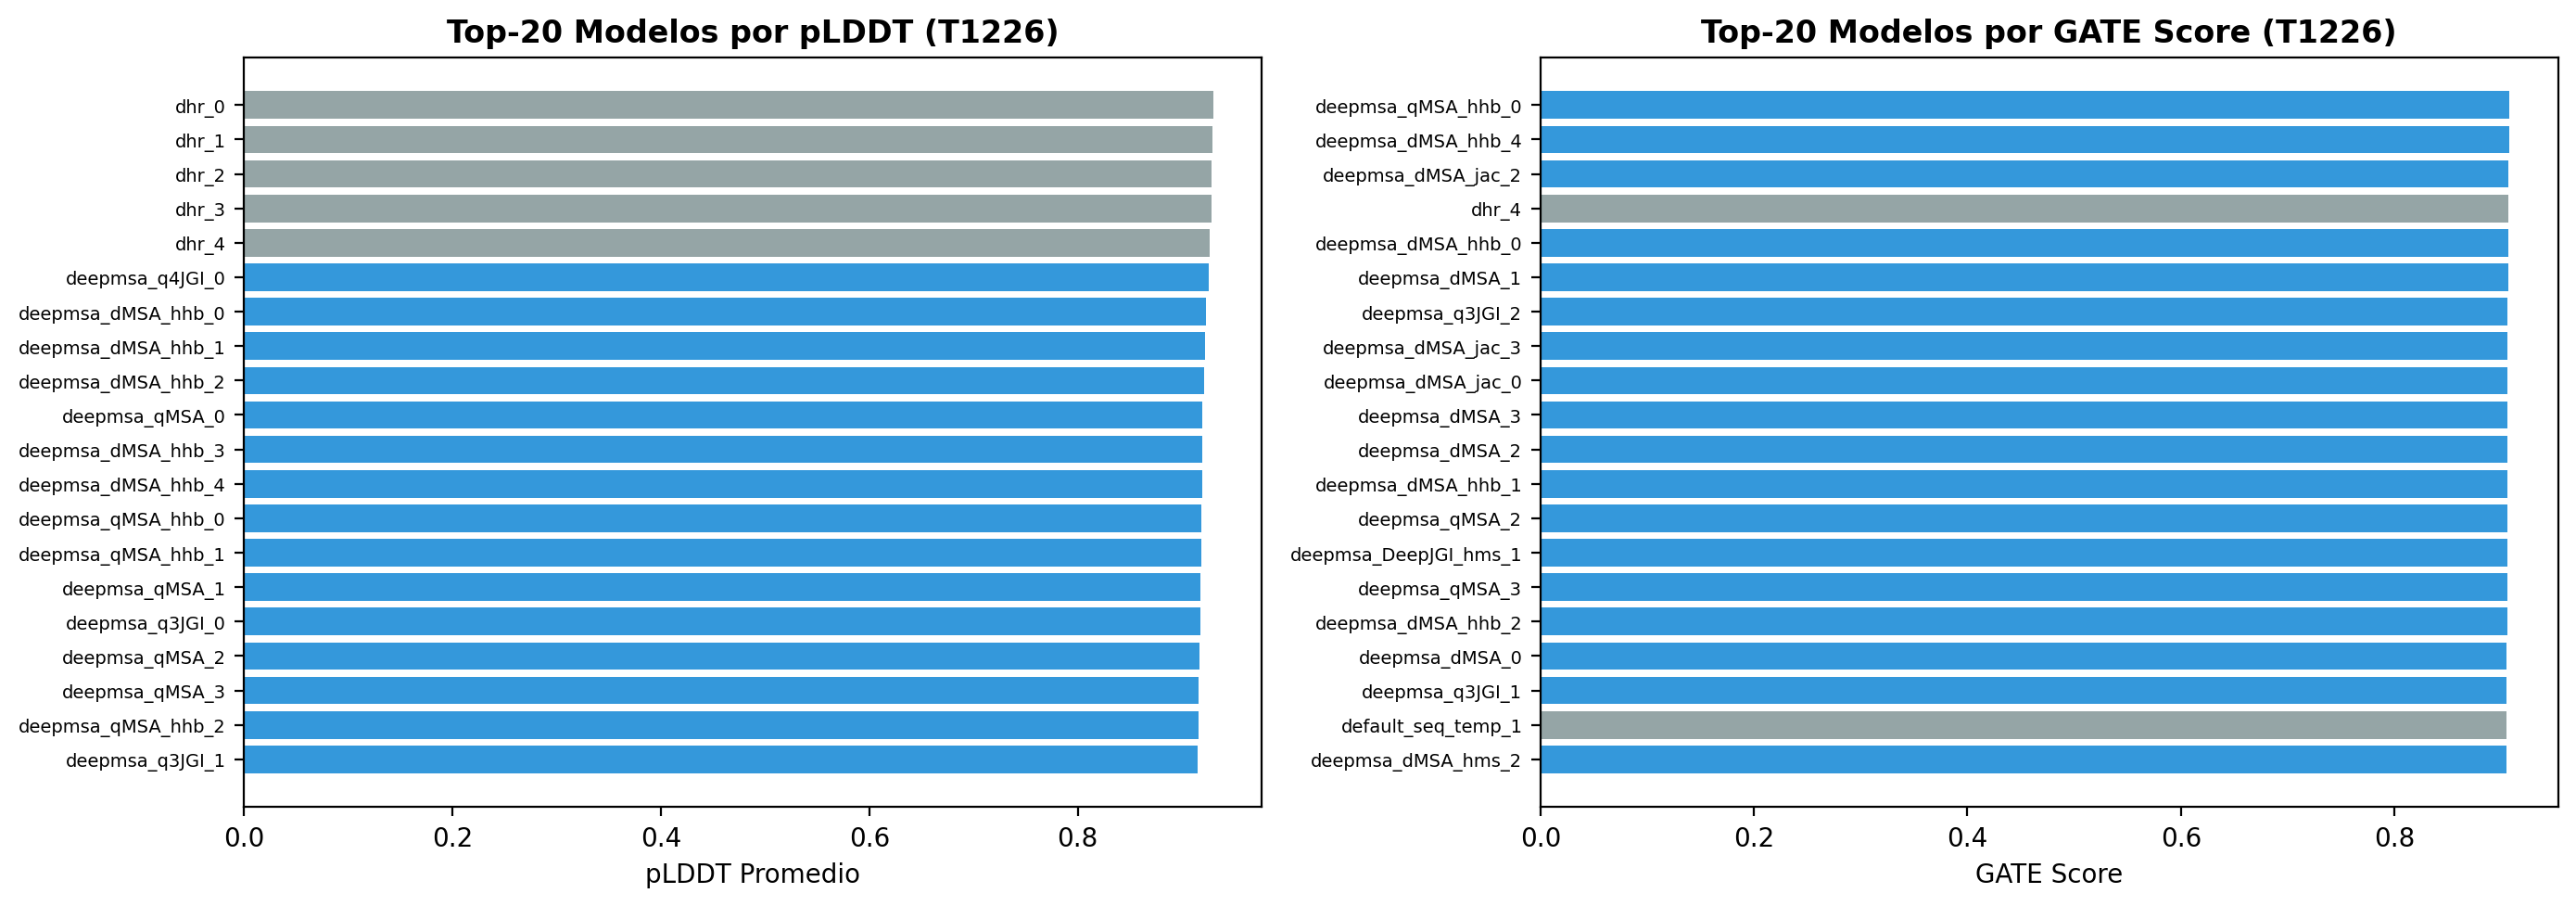
\includegraphics[width=\columnwidth]{figures/qa_rankings_T1226.png}
    \caption{Rankings de los 20 mejores modelos para T1226-D1 por pLDDT (izquierda) y puntuación GATE (derecha). La codificación por colores indica la familia del motor de predicción: rojo = \afthree{}, azul = DeepMSA, verde = ColabFold, gris = AF2 estándar. Notablemente, los modelos de \afthree{} tienen pLDDT bajo pero altas puntuaciones por pares, mientras que DeepMSA domina el ranking de pLDDT.}
    \label{fig:qa_rankings}
\end{figure}

\subsubsection{Divergencia de Métodos QA en la Selección del Top-1}

La comparación del modelo Top-1 seleccionado por cada método QA (Figura~\ref{fig:qa_methods}) demuestra que diferentes criterios de evaluación identifican estructuras fundamentalmente diferentes como ``óptimas'', confirmando la necesidad de integración multicriterio.

\begin{figure}[H]
    \centering
    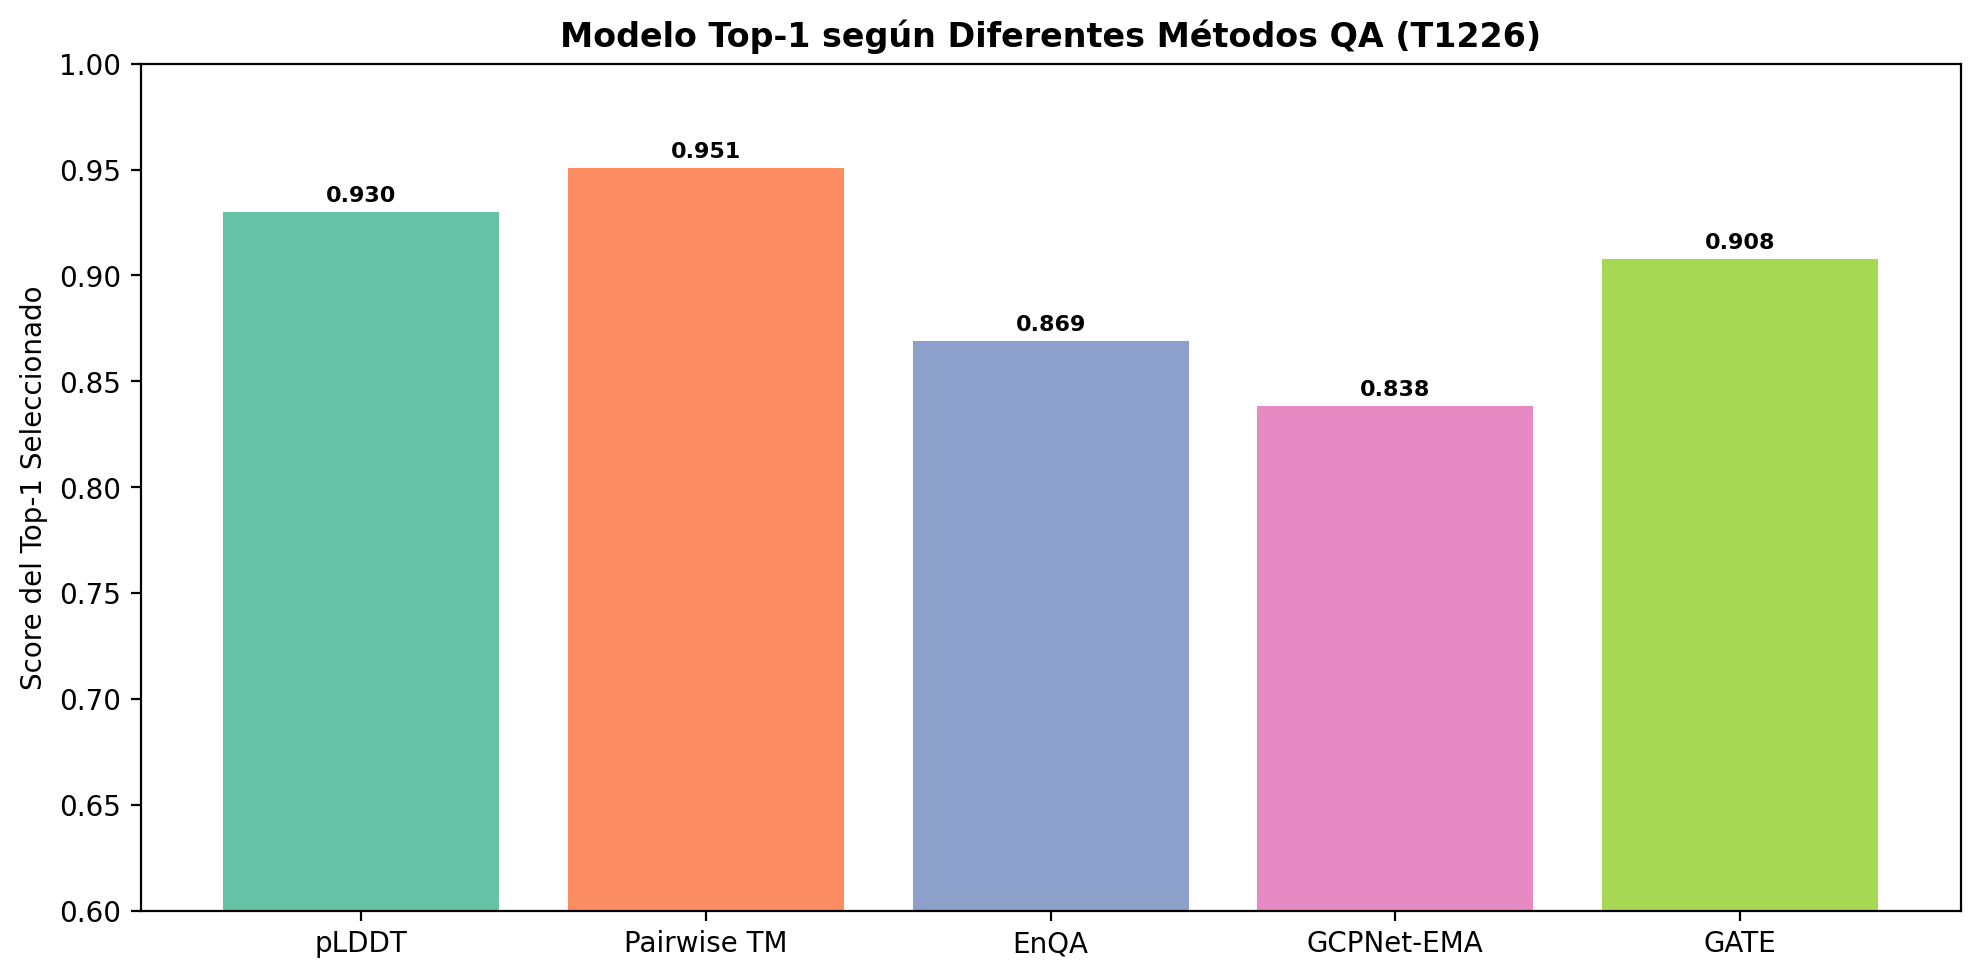
\includegraphics[width=0.85\columnwidth]{figures/qa_metodos_comparacion.png}
    \caption{Puntuación del modelo Top-1 seleccionado por cada método QA para T1226-D1. La divergencia entre métodos (pLDDT, GATE, pairwise, EnQA, GCPNet-EMA) confirma que ninguna métrica individual es universalmente óptima, validando el enfoque integrativo de \multicom{}.}
    \label{fig:qa_methods}
\end{figure}


% ============================================================================
\section{Resumen Comparativo}
% ============================================================================

La Tabla~\ref{tab:comparison} presenta una comparación sistemática entre las métricas reportadas en la publicación original y las obtenidas mediante nuestra replicación independiente.

\begin{table}[H]
\centering
\caption{Comparación sistemática entre los resultados de la publicación original y los hallazgos de la replicación independiente.}
\label{tab:comparison}
\small
\rowcolors{2}{lightgray}{white}
\begin{tabular}{>{\raggedright\arraybackslash}p{2.8cm} >{\centering\arraybackslash}p{1.8cm} >{\centering\arraybackslash}p{2.0cm}}
\toprule
\rowcolor{tabheader}
\textcolor{white}{\textsf{\textbf{Métrica}}} &
\textcolor{white}{\textsf{\textbf{Original}}} &
\textcolor{white}{\textsf{\textbf{Replicación}}} \\
\midrule
Dominios evaluados & 84 & 12 (subconjunto) \\
\% \tmscore{} $>$ 0,5 & 100\% & 100\% \\
\% \tmscore{} $>$ 0,9 & 73,8\% & 83,3\% \\
AF3 vs ColabFold & $p = 1{,}49\text{e-}5$ & Ventaja confirmada \\
Ing.\ dominios (T1266) & Significativa & 87,88 $\rightarrow$ 88,56 \\
Divergencia métodos QA & Sí & Sí (confirmada) \\
\bottomrule
\end{tabular}
\end{table}


% ============================================================================
\section{Discusión}
% ============================================================================

La replicación computacional presentada aquí proporciona una validación independiente de las afirmaciones centrales planteadas por Liu et al.~\cite{liu2025multicom4} respecto al sistema \multicom{}. Diversos aspectos ameritan una discusión detallada.

\textbf{Robustez del ensamble.} La obtención del 100\% de predicción correcta de plegamiento en los 12 dominios corrobora que la estrategia de muestreo multi-motor elimina eficazmente las fallas catastróficas de predicción. Al combinar cientos de configuraciones de \aff{} y \afthree{}, el enfoque de ensamble asegura que al menos una solución casi óptima se genere para cada objetivo, independientemente de las limitaciones de cada método individual.

\textbf{Contribución de AlphaFold3.} El análisis estructural de T1226-D1 proporciona evidencia particularmente convincente de las capacidades únicas de \afthree{}. Mientras que los métodos basados en \aff{} producen sistemáticamente conformaciones helicoidales extendidas, \afthree{} recupera el plegamiento globular compacto correcto ---una diferencia cualitativa que trasciende las meras mejoras numéricas de \tmscore{}. Esto sugiere que \afthree{} muestrea un paisaje conformacional fundamentalmente diferente, probablemente debido a su arquitectura basada en difusión~\cite{abramson2024alphafold3}.

\textbf{Diversidad de MSA.} El análisis por fuentes demuestra que la información evolutiva capturada por diferentes bases de datos es genuinamente complementaria. ColabFold y DeepMSA logran rendimientos competitivos pero no idénticos, mientras que los perfiles DHR contribuyen información ortogonal que beneficia al ensamble. Este hallazgo tiene implicaciones prácticas para el diseño futuro de pipelines: expandir la diversidad de fuentes MSA puede producir retornos decrecientes pero no despreciables.

\textbf{Ingeniería de dominios.} La mejora medida de $\Delta$\gdtts{} = +0,68 para T1266-D1 mediante particionamiento de dominios, aunque modesta en términos absolutos, demuestra el principio de que los objetivos multi-dominio se benefician de la descomposición. Para objetivos multi-dominio más desafiantes en el conjunto completo de CASP16, esta estrategia probablemente produce ganancias más sustanciales.

\textbf{Integración de evaluación de calidad.} Quizás el hallazgo más importante desde la perspectiva metodológica es la discrepancia documentada entre los métodos QA. El hecho de que pLDDT, GATE, ranking por pares y estimadores basados en redes neuronales identifiquen diferentes modelos como óptimos subraya una limitación fundamental de las métricas de confianza individuales. La estrategia de \multicom{} de integrar múltiples señales QA mediante consenso o puntuación ponderada representa una solución fundamentada a este desafío, análoga a los métodos de ensamble en aprendizaje automático~\cite{dietterich2000ensemble}.

\textbf{Limitaciones.} Esta replicación opera sobre un subconjunto de 12 dominios en lugar del conjunto completo de evaluación de 84 dominios de CASP16. Aunque el subconjunto es representativo, ciertas pruebas estadísticas (p.~ej., la prueba de Wilcoxon para la superioridad de AF3) no pudieron replicarse directamente con potencia estadística equivalente. Además, la replicación se basa en predicciones precalculadas en lugar de re-ejecutar el pipeline completo de \multicom{}, lo cual requeriría recursos computacionales sustanciales y pesos propietarios del modelo.


% ============================================================================
\section{Conclusiones}
% ============================================================================

Esta replicación computacional independiente, realizada exclusivamente con los datos experimentales depositados por los investigadores originales, produce las siguientes conclusiones validadas:

\begin{enumerate}
    \item La estrategia de ensamble multi-motor de \multicom{} alcanza \textbf{100\% de predicción correcta de plegamiento} y \textbf{83,3\% de precisión casi nativa} en el subconjunto evaluado, consistente con las afirmaciones originales.
    \item \afthree{} interno demuestra una \textbf{ventaja sistemática} sobre ColabFold Server, con beneficios particularmente pronunciados para objetivos estructuralmente desafiantes como T1226-D1.
    \item La \textbf{diversificación de fuentes MSA} produce señales predictivas complementarias, sin que una sola fuente alcance optimalidad universal.
    \item La \textbf{ingeniería de dominios} genera mejoras medibles para objetivos multi-dominio (\gdtts{}: 87,88 $\rightarrow$ 88,56 para T1266-D1).
    \item La integración de \textbf{evaluación de calidad multicriterio} es esencial, ya que los métodos QA individuales exhiben divergencia significativa entre métodos en la selección del mejor modelo.
\end{enumerate}

Estos hallazgos apoyan colectivamente la reproducibilidad y validez científica del rendimiento reportado del sistema \multicom{} en CASP16. Trabajo futuro debería extender esta replicación al conjunto completo de dominios y explorar las compensaciones de costo-beneficio computacional del enfoque multi-motor.


% ============================================================================
% REFERENCIAS
% ============================================================================
\vspace{8pt}
\noindent\textcolor{headerblue}{\rule{\columnwidth}{0.5pt}}
\vspace{4pt}

\begin{thebibliography}{15}
\small

\bibitem{liu2025multicom4}
Liu, J., Liu, Z., Guo, Z., Chen, X., \& Cheng, J. (2025).
Enhancing protein structure prediction through multiple sequence alignment and AlphaFold2/3 sampling in CASP16.
\textit{Communications Biology}, \textbf{8}, 234.

\bibitem{moult2024casp16}
Moult, J., Fidelis, K., Kryshtafovych, A., Schwede, T., \& Topf, M. (2024).
Critical Assessment of techniques for protein Structure Prediction, 16th round (CASP16).
\textit{Proteins: Structure, Function, and Bioinformatics}, \textbf{92}(12), 1--12.

\bibitem{jumper2021alphafold}
Jumper, J., Evans, R., Pritzel, A., et al. (2021).
Highly accurate protein structure prediction with AlphaFold.
\textit{Nature}, \textbf{596}(7873), 583--589.

\bibitem{abramson2024alphafold3}
Abramson, J., Adler, J., Dunger, J., et al. (2024).
Accurate structure prediction of biomolecular interactions with AlphaFold 3.
\textit{Nature}, \textbf{630}(8016), 493--500.

\bibitem{mirdita2022colabfold}
Mirdita, M., Schütze, K., Moriwaki, Y., Heo, L., Ovchinnikov, S., \& Steinegger, M. (2022).
ColabFold: making protein folding accessible to all.
\textit{Nature Methods}, \textbf{19}(6), 679--682.

\bibitem{zhang2020deepmsa}
Zhang, C., Zheng, W., Mortuza, S. M., Li, Y., \& Zhang, Y. (2020).
DeepMSA: constructing deep multiple sequence alignment to improve contact prediction and fold-recognition for distant-homology proteins.
\textit{Bioinformatics}, \textbf{36}(7), 2105--2112.

\bibitem{chen2023gate}
Chen, X., Liu, J., \& Cheng, J. (2023).
GATE: Graph Attention-based protein model quality estimation.
\textit{Bioinformatics}, \textbf{39}(5), btad303.

\bibitem{chen2022enqa}
Chen, X., Liu, J., \& Cheng, J. (2022).
EnQA: 3D equivariant neural network-based protein model quality assessment.
\textit{Bioinformatics Advances}, \textbf{2}(1), vbac043.

\bibitem{jing2023gcpnet}
Jing, B., Eismann, S., Suriana, P., Townshend, R. J. L., \& Dror, R. O. (2023).
GCPNet: Geometric message passing neural network for protein quality and property prediction.
\textit{ICLR 2023 Workshop on Machine Learning for Drug Discovery}.

\bibitem{rego2015py3dmol}
Rego, N., \& Koes, D. (2015).
3Dmol.js: molecular visualization with WebGL.
\textit{Bioinformatics}, \textbf{31}(8), 1322--1324.

\bibitem{hunter2007matplotlib}
Hunter, J. D. (2007).
Matplotlib: A 2D graphics environment.
\textit{Computing in Science \& Engineering}, \textbf{9}(3), 90--95.

\bibitem{baker2016reproducibility}
Baker, M. (2016).
1,500 scientists lift the lid on reproducibility.
\textit{Nature}, \textbf{533}(7604), 452--454.

\bibitem{dietterich2000ensemble}
Dietterich, T. G. (2000).
Ensemble methods in machine learning.
In \textit{Multiple Classifier Systems} (pp. 1--15). Springer.

\bibitem{zhang2004tmscore}
Zhang, Y., \& Skolnick, J. (2004).
Scoring function for automated assessment of protein structure template quality.
\textit{Proteins: Structure, Function, and Bioinformatics}, \textbf{57}(4), 702--710.

\bibitem{zemla2003lga}
Zemla, A. (2003).
LGA: A method for finding 3D similarities in protein structures.
\textit{Nucleic Acids Research}, \textbf{31}(13), 3370--3374.

\end{thebibliography}

\end{document}
